\let\textcircled=\pgftextcircled
\chapter {Estimación del tiempo de viaje}
\label{chap:estimacion}

A fin de definir el problema es necesario introducir los siguientes componentes:

\textbf{Una red espacial digital} es un grafo \(\mathcal{G <V,E>}\) donde \(\mathcal{V}\) es un conjunto de vértices y \(\mathcal{E}\) un conjunto de arcos. Cada arco tiene las propiedades: vértices, longitud, dirección. Adicionalmente, una red tiene propiedades relacionadas al tránsito, como restricciones de giro, límites de velocidad, información de semáforos, etc.

\textbf{Un conjunto de datos de localización} consiste de: (a) latitud, (b) longitud, (c) tiempo del muestreo, (d) identificación del dispositivo. La ubicación  reportada por un dispositivo es también llamada sonda. Una secuencia de sondas provenientes de un mismo vehículo se denota por \(\mathcal{P} = p_1,p_2,...,p_{t-1}\).

\textbf{Una trayectoria real} es una secuencia de arcos que representan el camino real atravesado por un vehículo a medida que se generan las observaciones \(\mathcal{P}\). Es denotada por \(\mathcal{T}\) y no es considerada en el contexto de map-matching (excepto como datos ground truth).

\textbf{Una trayectoria observada} es una secuencia de segmentos de línea recta, tal que cada línea conecta dos posiciones observadas consecutivas.

El problema es entonces definido como: buscar la secuencia de arcos más probable ($\tau_{opt}$) para una secuencia de observaciones \(\mathcal{P}\) y una red espacial digital  \(\mathcal{G}\):
\[\tau_{opt} = arg \max_{\tau} \mathbb{P}(\tau = \mathcal{T|P,G})\] 
donde \( \mathbb{P}(\tau = \mathcal{T|P,G})\) es la probabilidad ser $\tau$ la verdadera trayectoria dado \(\mathcal{P}\) y \(\mathcal{G}\).

\section{Estimación de la trayectoria}
Asumiendo que un dispositivo viaja a través de una red espacial de calles o caminos, el objetivo es producir una estimación segundo a segundo de su ubicación en base a una serie de transmisiones de cada dispositivo. Esta tarea presenta los siguientes desafíos: 

\textbf{Consumo de energía:} En este caso se considerará la dispersión espacial de detecciones, es decir, es deseable partir de observaciones que se realizan con baja periodicidad, ya que una alta periodicidad en las transmisiones implica mayor consumo energético del dispositivo. Esto hace que métodos estándar basados en triangulación no sean aptos. 

\textbf{Muestras de baja precisión:} Incluso cuando el consumo de energía no es una preocupación, los sensores GPS no siempre están disponibles. Algunos celulares usan WiFi y la señal de celular para el posicionamiento, siendo este de menor calidad. Incluso las experiencias con GPS pueden no ser las esperadas, por ejemplo, cuando el usuario se encuentra con el celular en el bolsillo o está atravesando zonas de edificios de gran altura o túneles donde la precisión se reduce a decenas o cientos de metros.

\subsection{Solución trivial}
Considere la siguiente solución:

\begin{adjustwidth}{2cm}{}
\textbf{
Al realizar una observación, tomar la posición de menor distancia al segmento de calle más cercano al origen de la transmisión. Interpolar las ubicaciones entre observaciones.
}
\end{adjustwidth}

En primer lugar, utilizar el segmento más cercano a cada posición frecuentemente no es el segmento real por donde circula un vehículo. En segundo lugar, las variaciones en el muestreo por error de los instrumentos de posicionamiento aumentan la complejidad en situaciones de dispositivos estacionarios, donde pueden ocurrir observaciones intermitentes.  En el algoritmo planteado, esto se refleja como saltos entre las ubicaciones, ubicando las detecciones en posiciones hacia delante y hacia atrás. \par Por último, interpolar ubicaciones distantes por línea recta producen trayectorias de baja calidad. El uso de una red espacial, como el mapa de una ciudad puede mejorar significativamente el resultado, pero introduce ambigüedades en las rutas que deben ser resueltas.
Utilizar el camino más corto entre las muestras no es aplicable por la alta incertidumbre de la ubicación.
Como se sugiere en este ejemplo, soluciones por algoritmos determinísticos no se ajustan al problema, debido a la naturaleza estocástica de las detecciones.

\subsection{Algoritmo básico de estimación de trayectoria}
A continuación se presenta un método probabilístico para la estimación de la trayectoria. En lugar de asociar el segmento más cercano a una observación en cada instante de tiempo, se modela la distribución de posibles ubicaciones a lo largo del tiempo, y se toma la trayectoria que maximiza la probabilidad en el modelo. \par
Para reducir el conjunto de ubicaciones posibles y restricciones de movimiento, se asume que el dispositivo viaja a través de una red espacial conocida. El modelo, tomado como entrada del algoritmo, consiste en vértices localizados espacialmente, conectados por arcos dirigidos. \par
Dada la red espacial, el problema de estimación de trayectoria tiene cierta similitud con map-matching, que busca coincidir una secuencia de observaciones escasas y ruidosas con una serie de estimaciones de ubicación. Nuestro método está basado en map-matching de Viterbi.  \par
Formulamos el problema usando Modelos Ocultos de Markov para estados, probabilidades de transición y probabilidades de emisión, utilizando decodificación por el algoritmo de Viterbi para determinar la trayectoria más probable, representada por una secuencia de estados ocultos en el Modelo de Markov.
Utilizado en conjunto con el algoritmo de Viterbi, un Modelo Oculto de Markov espera una entrada periódica y produce una transición de estados $i\rightarrow j$ por período. Las transiciones son regidas por probabilidades de transición $p(i\rightarrow j)$, y probabilidades de emisión $p(obs|i)$, donde $obs$ es la observación actual. Las auto-transiciones son permitidas. A continuación se describe en detalle la formulación de los Modelos Ocultos de Markov.

\subsection{Modelos ocultos: Segmentos de calles}\label{ssec:hmm-shortsegments}

Un mapa de calles simple consiste de vértices representando las intersecciones, arcos representando los segmento de una calle, y (mayormente para vehículos) restricciones de giro que determinan las transiciones permitidas entre arcos.

Nuestro modelo debe ser capaz de reconocer el trayecto más probable segundo a segundo siendo este un trayecto válido. Para esto, es necesario contar con estados de extensión espacial significativamente menor al segmento de una calle o cuadra, las cuales pueden superar los cientos de metros (Figura \ref{fig:segmentos-cortos}). 


\begin{figure}[!htp]
	\centering
	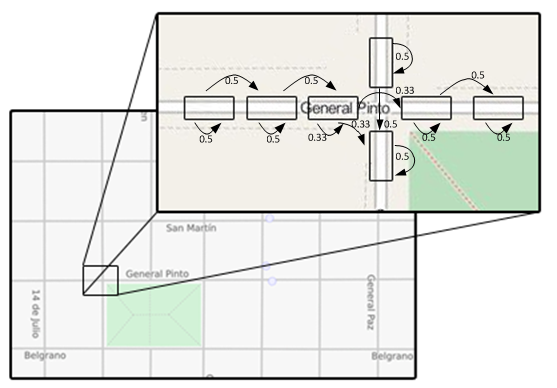
\includegraphics[width=0.5\textwidth]{images/segmentos_cortos.png}
	\captionsetup{width=.6\linewidth}
    \caption{Modelo oculto de Markov de dos calles intersectadas. Los segmentos son sub-divididos para aumentar la granuralidad}
    \label{fig:segmentos-cortos}
\end{figure}

Cada estado representa un área rectangular en la cual puede estar ubicado un emisor GPS. Una calle puede ser atravesada pasando por todos los segmentos, sin saltos entre segmentos no adyacentes. Se mantienen las restricciones de giro para el último segmento de cada cuadra.

De esta forma definimos \(\mathcal{G'=<V',E'>}\) como un nuevo grafo compuesto por los segmentos, con estados como vértices y transiciones basadas en las restricciones de giro como arcos.

\subsection{Probabilidades de transición}

Las probabilidades de transición reflejan los siguientes conceptos: 1) Para un segmento dado, existe una probabilidad de que en el siguiente instante, el vehículo se encuentre en ese mismo segmento. 2) Un vehículo puede viajar solo del final de un segmento al comienzo del siguiente si usa la misma intersección; esto asegura que el camino de segmentos saliente sea contínuo. 3) Un vehículo no puede viajar irrazonablemente rápido en cualquier segmento. En otras palabras, las transiciones modelan el comportamiento en las intersecciones: continuando o girando. Se usan probabilidades uniformes entre segmentos adyacentes. Por lo tanto, para cada segmento $i$, con segmentos adyacentes $n \in N$, $p(i\rightarrow i) = p(i\rightarrow n)= \frac{1}{|N|+1} $. Todas las restricciones, incluyendo las permitidas y las prohibidas, son contadas en los segmentos adyacentes.

\subsection{Probabilidades de emisión}\label{ssec:emission}

Describe la probabilidad $p(obs|s)$ de hacer una observación $obs$ en el estado actual $s$.

Una observación $obs$ consiste en un nuevo punto $p_i$ (lat,lng) de la trayectoria $\mathcal{P}$. Para cada segmento candidato $n \in N$ se modela la probabilidad de emisión como una función de distribución normal que depende de la distancia del segmento a la observación $p_i$. Concretamente, la densidad de probabilidad de emisión para el segmento $i$ con la observación $p$ es $N(\mathrm{dist}(i,p))$, donde N es una función Gaussiana bivariada con media en el centro del segmento, y $\mathrm{dist}(i,p)$ es la distancia Euclideana entre $i$ y $p$. La varianza de $N$ depende del tipo de sensor (A-GPS/WiFi/Celular). Se toma como referencia un error de 10 metros (medido en estudios previos sobre precisión de sistemas de posicionamiento en dispositivos móviles \cite{jones2015horizontal}).
Este modelo representa el concepto de que es probable que un punto particular haya sido observado desde un segmento próximo, pero no necesariamente el más cercano.

Adicionalmente, se introducen dos métodos que permiten calcular $p(obs|s)$ considerando a cada segmento como un punto (método 1), o como una superficie (método 2). Se utiliza la ecuación \eqref{eq:distancia} que describe valores bajos al aumentar las distancias.  \par

\begin{align}\label{eq:distancia}
 p(obs|s)= \frac{e^{-d((x,y);X_j)^2}}{\sum\limits_{k=1}e^{-d((x,y);X_k)^2}} 
\end{align}

\subsubsection{Método 1}\label{sssec:metodo1}
Para cada observación $p_i$ se calcula la distancia entre cada segmento y la observación. La ubicación del segmento se corresponde con el centroide de la superficie que lo define. Se aplica un factor de corrección sobre la distancia para escalar los valores pequeños provenientes de las distancias geodésicas expresadas en Km. El valor que se devuelve es $p(obs|s)$

\algnewcommand\algorithmicforeach{\textbf{for each}}
\algdef{S}[FOR]{ForEach}[1]{\algorithmicforeach\ #1\ \algorithmicdo}

\begin{algorithm}
\caption{Método 1}\label{metodo1}
\begin{algorithmic}[1]

\Procedure{probability}{$p_i$}
\State $pow\gets e^{-distancia(p_i,centroide)^2}$
\ForEach {$s \in \mathcal S $} \Comment{Normalización}
\State $norm\gets norm + e^{-distancia(p_i,s)^2}$

\EndFor
\State \textbf{return} $pow/norm$
\EndProcedure

\end{algorithmic}
\end{algorithm}

\subsubsection{Método 2}\label{sssec:metodo2}
A diferencia del método 1, se considera la superficie del segmento en el cálculo de $pow$. Se calcula la suma de $e^{{-d}^2}$ sobre el área de cada segmento. Se aproxima sobre la superficie dividida en intervalos pequeños con una separación  ($\delta x, \delta y$), mas precisamente, la décima parte del tamaño de cada segmento en x e y 

\begin{algorithm}
\caption{Método 2}\label{metodo2}
\begin{algorithmic}[1]
\Procedure{pow}{$p_i$,s}
  \For{\texttt{$x \gets xMin;x < xMax; x+\delta x$}}
    \For{\texttt{$y \gets yMin;y < yMax; y +\delta y$}}
		\State $ centroide \gets Point(x,y) $
        \State $pow\gets pow+ e^{-distancia(p_i,centroide)^2}$
    \EndFor
  \EndFor
  \State \textbf{return} $pow$
\EndProcedure

\end{algorithmic}
\end{algorithm}


\subsection{Algoritmo de Viterbi}
\label{ssec:algoritmo-viterbi}

Dado un HMM y un conjunto de observaciones $obs$, se extrae la trayectoria que maximiza la probabilidad de las observaciones en el modelo.
El Modelo Oculto de Markov estará definido por los estados, el vector de probabilidades iniciales $\pi_i$ para cada estado, la matriz de probabilidades de transición $a$, y un vector de funciones de distribución de probabilidades de observaciones $opdfs$.

\textbf{$\pi$} Valores de probabilidad inicial, $\pi_i$ es la probabilidad inicial del estado $i$.

$\textbf{a}$ Un arreglo de probabilidades de transición de estados. $a_{ij}$ es la probabilidad de ir desde el estado $i$ al estado $j$.

$\textbf{opdfs}$ Son las distribuciones de observación, $opdfs[i]$ es la distribución de observación asociada al estado $i$.

Serán tantos estados como segmentos existan en la red espacial definida  $\mathcal{G'}$. Para construir el modelo, se itera sobre los segmentos definidos en \(\mathcal{G'}\) y se crea un estado para cada segmento, con probabilidad $pi_i = \frac{1}{cant(segmentos)}$. 

Una distribución $opdf$ está dada por una función de distribución normal bivariada con media en el centroide del segmento $s$, $\mu = (avg(longitud),avg(latitud))$ y la matriz identidad como matriz de covarianza. $A_{ij}$ estará dado por $\frac{1}{(d_{max}+1)}$, donde $d_{max}$ es el grado máximo saliente para $s$, incluyendo la auto-transición de cada estado.
En la Figura \ref{fig:opdf} se ejemplifica la función de distribución para un segmento $s'$ con centroide $\mu'= (a,b)$. Se observa la variación de la probabilidad $p(obs|s')$ en función de la distancia respecto a $\mu'$. Los métodos 1 y 2 definidos en la sección \ref{ssec:emission} se presentan como alternativas a la función de distribución normal bivariada.

\begin{figure}[!htp]
	\centering
	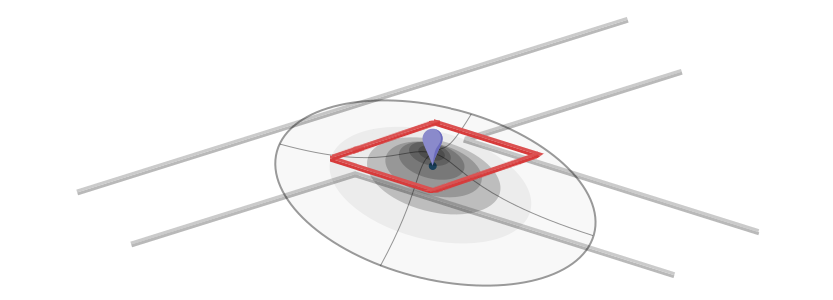
\includegraphics[scale=0.5]{images/gaussian-sq.png}
    \caption{Función de densidad de probabilidades bidimensional.}
    \label{fig:opdf}
\end{figure}

La decodificación por Viterbi es una técnica de programación dinámica para buscar la secuencia de estados ocultos más probable dado un conjunto de observables y la distribución de probabilidades de emisión y probabilidades de transición. En nuestro caso, los estados ocultos se corresponden con la trayectoria recorrida, y los observables son las muestras de posición.

\subsubsection{Ejemplo HMM}
En la Figura \ref{fig:momex} se muestra un ejemplo donde S1, S2, y S3 son segmentos de calle y p1, p2, p3, y p4 son observaciones realizadas. Hay igual probabilidad de hacer una transición desde S1 a S1, S2, o S3. Como la función de densidad de probabilidad de emisión es una función decreciente de la distancia, la secuencia de segmentos más probable para la secuencia de observaciones dada es S1, S3, S3, S3, y S3. Si bien p2 es más cercano a S2, el estado oculto más probable de ese punto es S3 dadas las restricciones de transitividad. Si se toma el camino atravesando S2, no es posible girar luego a S3.

\begin{figure}[H]
\centering
\begin{minipage}{.5\textwidth}
  \centering
  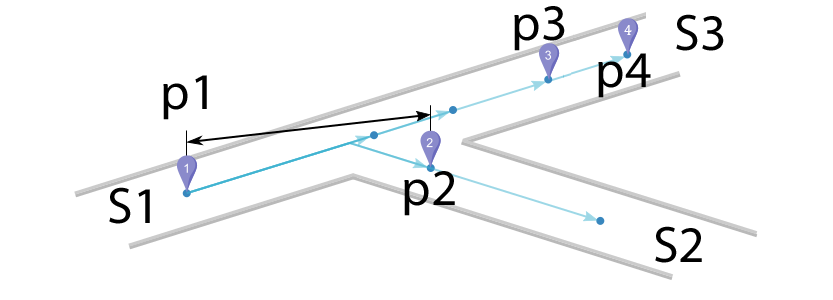
\includegraphics[width=1\linewidth]{images/detecciones.png}  
\end{minipage}%
\begin{minipage}{.5\textwidth}
  \centering
  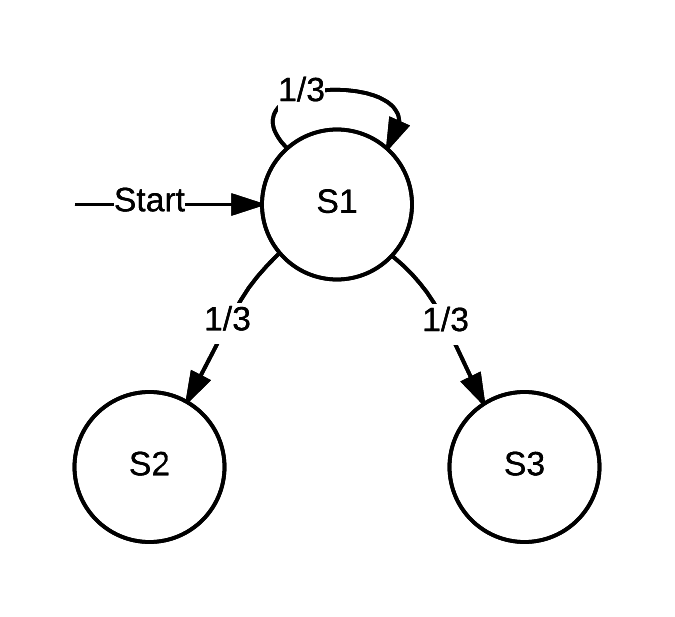
\includegraphics[width=0.5\linewidth]{images/mom-segmentos.png}  
\end{minipage}%
	\captionof{figure}{Ejemplo de HMM}
	\label{fig:momex}
\end{figure}

Es claro en este ejemplo la utilidad de HMM, es robusto frente a muestras posicionales cercanas a un segmento que no sea el correspondiente a la observación, y representa correctamente la idea de una ruta continua en lugar de una secuencia de segmentos.

\subsubsection{Flujo del algoritmo}
\begin{itemize}
\item Para cada punto de una trayectoria observada, se computa la probabilidad de emisión para cada segmento candidato (estados ocultos), representados por los círculos vacíos en la Figura \ref{fig:algviterbi}. Mientras que la probabilidad de transición es asignada a cada estado incidente en el estado oculto.\par
\begin{figure}[ht]
	\centering
	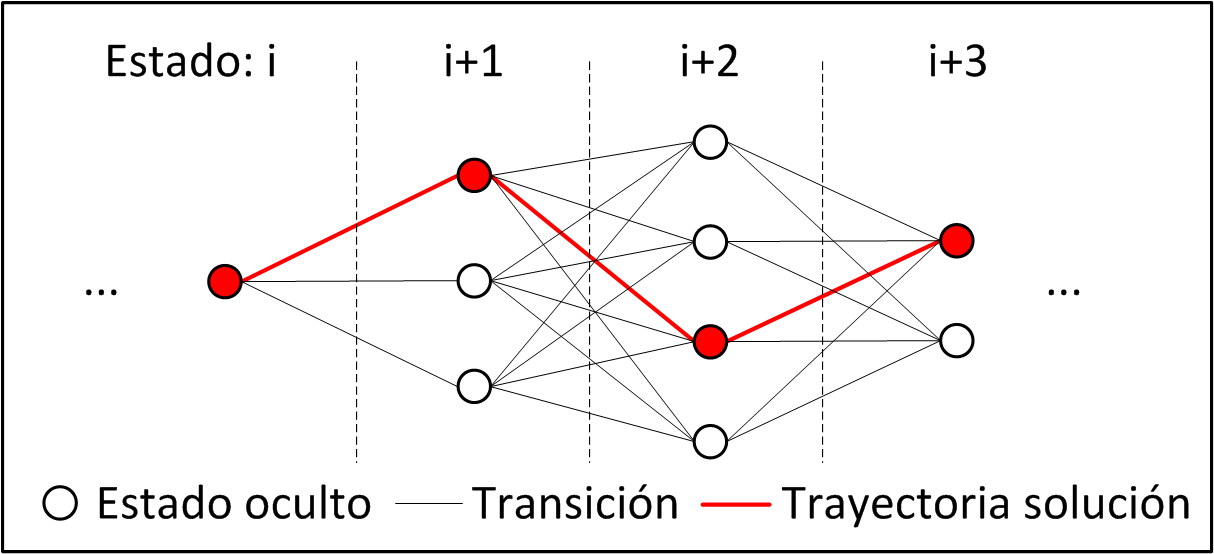
\includegraphics[scale=0.7]{images/viterbi.png}
    \caption{Diagrama de funcionamiento del algoritmo de Viterbi}
    \label{fig:algviterbi}
\end{figure}
\item El algoritmo realiza backtracking sobre la cadena de Markov actualizada y arroja una solución parcial.
\item El proceso anterior es repetido para el próximo punto de la trayectoria. El algoritmo termina cuando el último punto es alcanzado.
\end{itemize}


\section{Estimación a partir de dispositivos inalámbricos}\label{sec:estimacionwireless}

Aquí, $p(obs|s)$ describe la probabilidad de hacer una observación $obs$ si el estado actual es $s$, con la siguiente variación: una observación $obs$ consiste en un conjunto de detecciones del dispositivo en cuestión, por todos los monitores (detectores), en el tiempo actual. El modelo de probabilidades de emisión describe la distribución de probabilidades de la ubicación de un dispositivo en toda la red, para cada segundo.

En el caso de la localización basada en lecturas de señales provenientes de dispositivos inalámbricos, se busca que el modelo capture la relación estocástica entre la intensidad de señal y la distancia.

Las probabilidades de emisión se ven influenciadas por diversos factores, como por ejemplo la distancia, siendo este el de mayor interés. Intuitivamente, la probabilidad de hacer una detección decrece a medida que aumenta la distancia entre el dispositivo emisor y el monitor, alcanzando cero en el rango máximo de recepción. Por otro lado, la variabilidad del canal (\textit{fading}) también es un factor significativo, influenciado principalmente por la ubicación (el entorno) y los obstáculos presentes. Esto implica que una transmisión puede no ser detectada, incluso a corta distancia. 

Una observación $obs$ consiste de un conjunto de eventos $e_m \in  obs$, uno por cada monitor $m$, tal que:

\begin{align}\label{eq:observacion}
 p(obs|s)= p_{tx}\prod_{m \in obs}{p(e_m|s,tx)}
\end{align}

donde $tx$ indica que una transmisión ocurrió, y $p_{tx}$ es la probabilidad de que una transmisión esté ocurriendo. Se fijó $p_{tx}=0.97$, medido experimentalmente en reportes previos sobre identificación efectiva de dispositivos Bluetooth en distancias hasta 100 metros\cite{huang2014blueid}. Cabe aclarar que el método no es sensible a éste parámetro.

Cada evento $e_m$ puede tomar los valores $deteccion_m$ o $nodeteccion_m$, donde $nodeteccion_m$ indica que el dispositivo no fue detectado por ese monitor. Las \textit{no-detecciones} pueden no ser reportadas al servidor: la ausencia de una detección indica una no-detección. Cada $deteccion_m$ es acompañada de una intensidad de señal. 

Para todos los estados $s$, vale que $p(nodeteccion_m|s) = 1 - p(deteccion_m|s)$. Para estados fuera del alcance máximo de detección, es $p(deteccion_m|s) = 0$. 

\begin{figure}[!htp]
	\centering
	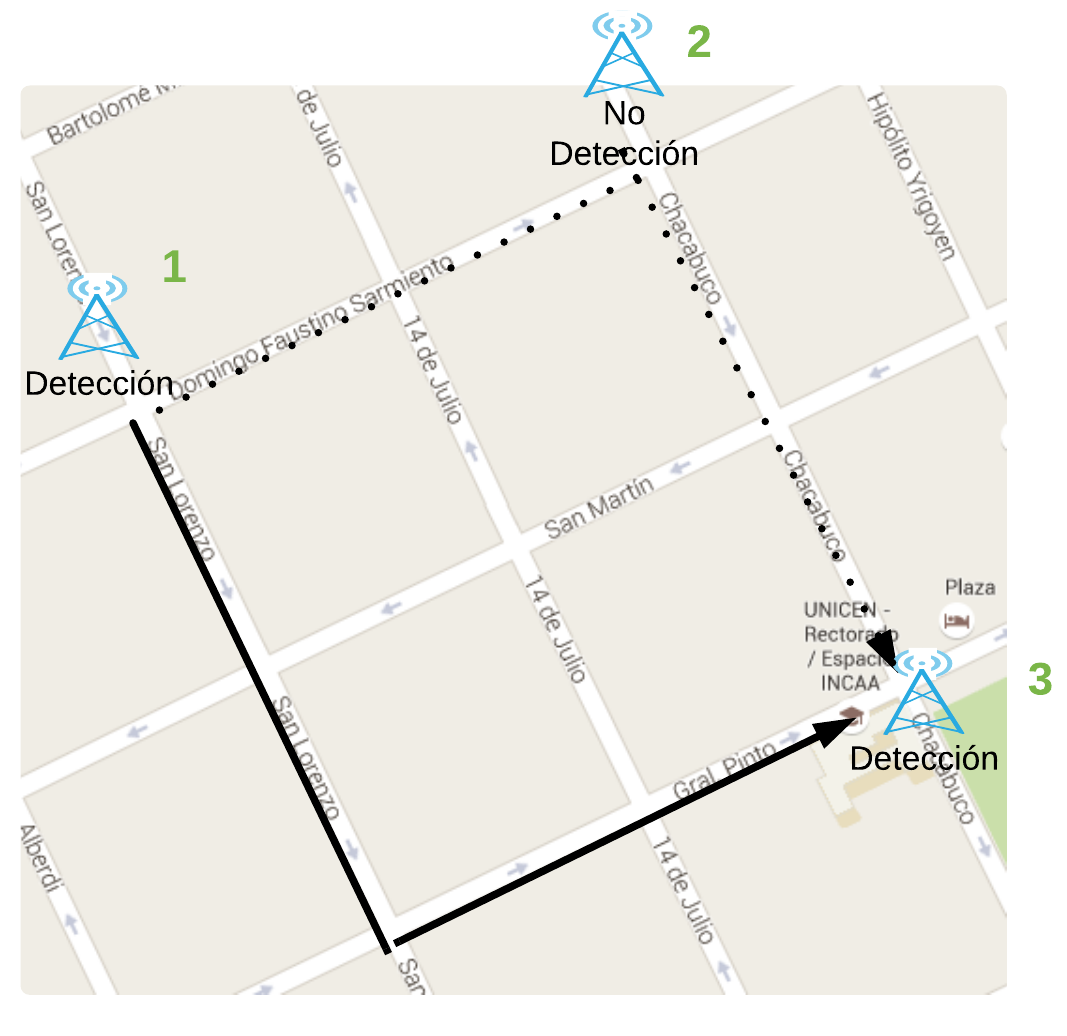
\includegraphics[scale=0.7]{images/motivating_example.png}
	\captionsetup{width=.7\linewidth}
	\caption{Ejemplo para diseño del modelo de emisión de probabilidades}
    \label{fig:motivating-example}
\end{figure}

La Figura \ref{fig:motivating-example} ilustra un ejemplo a partir del cual surge el modelo de emisión de probabilidades. Un dispositivo atraviesa el área de detección del monitor 1 y a continuación viaja a través de un camino desconocido sin ser detectado hasta el monitor 3. Aquí, el hecho de que ocurra una no-detección entre los monitores 1 y 3 aporta cierta información. Siendo que nos encontramos en igualdad de condiciones, es más probable que el dispositivo haya viajado sobre la ruta sin detectores intermedios.

Para determinar $p(deteccion_m|s,tx)$, nos basamos en medidas experimentales de la señal de radiofrecuencia, utilizando un vehículo y detectores Bluetooth (monitores). Para recolectar medidas se condujo a lo largo del alcance de detección de un monitor con el dispositivo Bluetooth encendido, registrando los paquetes transmitidos. Posteriormente se utilizó un estimador de funciones de densidad no paramétrico (método Kernel) sobre la distancia de los paquetes recibidos, o bien:

\begin{align}\label{eq:dist_given_rss}
 p(dist|RSS)= \sum_{dist \in paquetes_recibidos}{N(dist,\sigma^2).}
\end{align}

La Figura \ref{fig:opdf-kernel} ilustra, para un paquete recibido con una intensidad RSS dada, la densidad de probabilidad de la distancia en la que se encontraría el transmisor $p(dist|RSS)$. A valores de intensidad altos, hay mayor probabilidad de que un vehículo se encuentre a corta distancia (ej. entre 0 y 50 metros para un RSS $>-60$). En el caso opuesto, a menor intensidad, es mayor la incertidumbre sobre la distancia entre dispositivos (ej. valores por debajo de -70dB pueden provenir de cualquier ubicación en el área de cobertura del detector).

\begin{figure}[!htp]
	\centering
	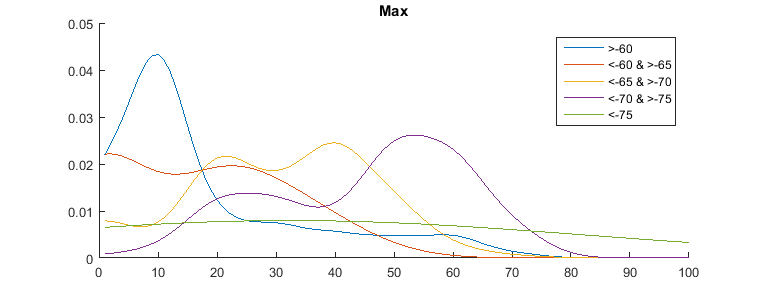
\includegraphics[width=0.9\textwidth]{images/selected-opdf.png}
	\caption{Funciones de densidad de probabilidad de observación Bluetooth}
    \label{fig:opdf-kernel}
\end{figure}

Definida la función de densidad de probabilidades, es posible calcular la probabilidad de hacer una detección $p(deteccion_m|s,tx)$ para un paquete de una intensidad de señal dada sobre la superficie que define al estado $s$:

\begin{align}
    \centering
    p(deteccion_m|s,tx) = \int_x \int_y p(dist(x,y,m)|RSS)\mathrm{d}x\mathrm{d}y
\end{align}

donde dist(x,y,m) es la distancia euclidea entre la coordenada $x,y$ y el monitor $m$.